\section{Δίκτυο Γεωμετρικής Ανακατασκευής και Χρωματικής Αποτύπωσης}
\label{idrnetwork}
\subsection{Συμβολισμοί}
Οι συμβολισμοί που συνοδεύουν τις παρακάτω αναλύσεις είναι οι εξής:
\begin{itemize}
    \item $u$ - Θέση pixel στην εικόνα
    \item $c$ - Θέση κάμερας
    \item $\hat{p}$ - Εκτιμώμενο σημείο στην επιφάνεια
    \item  $f_\theta$ - Νευρωνικό πεδίο προσημασμένης απόστασης SDF 
    \item $\mathcal{M}_\theta$ - Νευρωνικό πεδίο αποτύπωσης χρώματος στην εικόνα
    \item $\mathcal{L}_{u}(\theta, \gamma, \tau)$ - Πεδίο, έμμεσης διαφορίσιμης αποτύπωσης 
    \item $I, \hat{I}$ - Εικόνα και εκτίμηση εικόνας
    \item $S_\theta$ - Αναπαραστώμενη επιφάνεια
    \item $\boldsymbol{w}$ - Μοναδιαίο διάνυσμα πάνω στην ακτίνα με κατεύθυνση της κατεύθυνση όψης
    \item $R_u(t)$ - Παραμετρική εξίσωση ακτίνας που διέρχεται απο pixel $u$ και έχει παράμετρο $t$
    \item $\theta, \gamma, \tau$ - Παράμετροι βελτιστοποίησης
\end{itemize}

\subsection{ Διαφορίσιμη νευρωνική αποτύπωση σε  βήματα}
Προς το παρόν είδαμε, υπό γενική μορφή, πως αναπαρίστανται πολλαπλότητες μέσω νευρωνικών δικτύων αλλά και πως ελέγχονται οι διαφορίσιμες πολλαπλότητες. Στο παρόν κομμάτι παρουσιάζεται αναλυτικά πως αυτά εφαρμόζονται στην γενική περίπτωση ανακατασκευής επιφανειών με νευρωνικά δίκτυα, κάνοντας χρήση εικόνων ως κύριο μέσο επίβλεψης.
    Κατά το εμπρόσθιο πέρασμα του δικτύου αυτά που εκτελούνται είναι τα εξής:
    \begin{itemize}
        \item Για κάθε ενδιαφέρον pixel  \(u\) στην μάσκα της εικόνας \({I}\) που καλύπτει την περιοχή του αντικείμενου
        \item Βρες το σημείο \(\hat{p}\) πάνω στην ακτίνα \(w\) εκτελώντας Sphere Tracing με αφετηρία \(r_0\) 
        \item Εντός της επιφάνειας \(f_\theta \leq 0\), Εκτός της επιφάνειας \(f_\theta \geq 0\) 
        \item Για δεδομένο σημείο \(\hat{p}\) με εκτιμώμενη προσημασμένη απόσταση \( f( \hat{p})\)
        \item Υπολόγισε το χρώμα (Τexture Field) \(\mathcal{M_\theta}(\hat{p})\) στο σημείο \(\hat{p}\)
        \item Τοποθέτησε το χρώμα \(\mathcal{M_\theta}(\hat{p})\) στο pixel \(u\) 
    \end{itemize}
    \begin{figure}[ht]
    \centering
    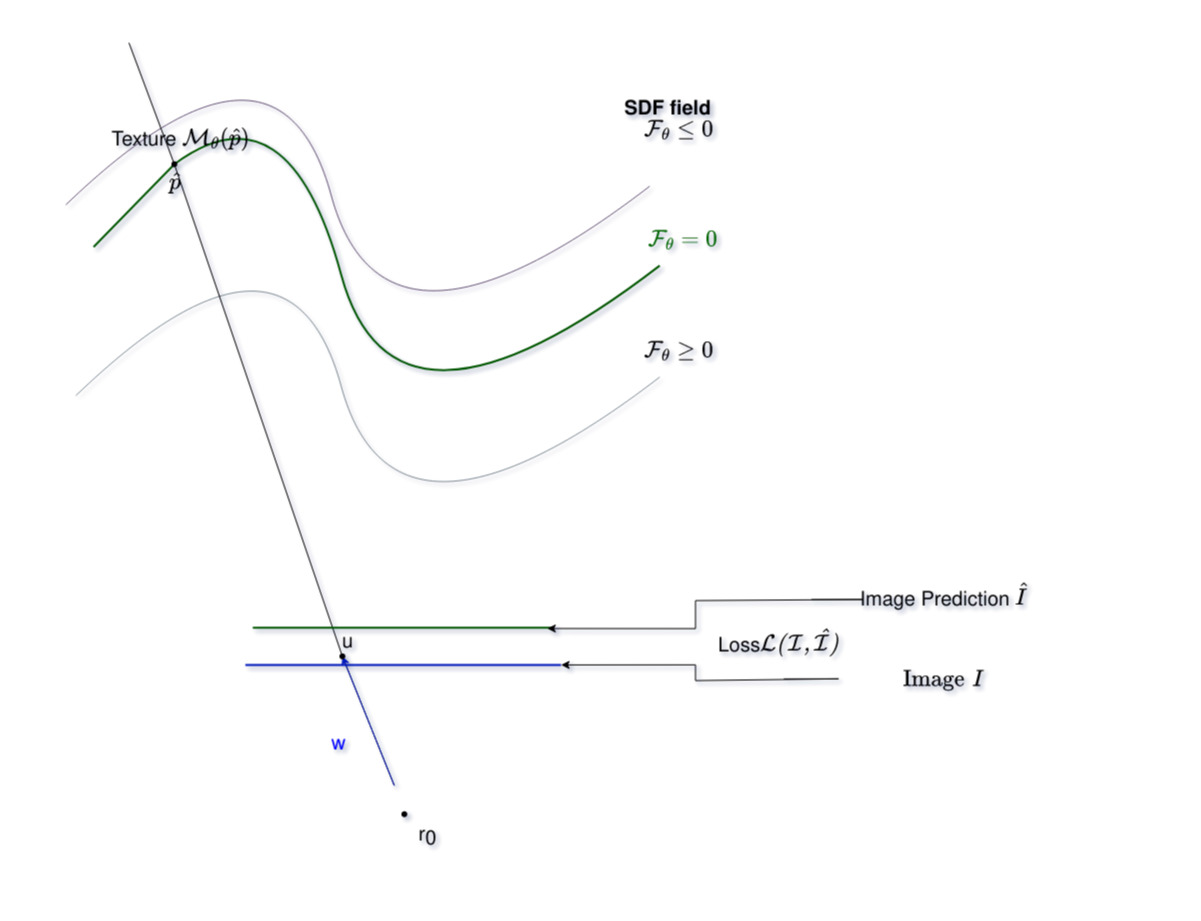
\includegraphics[width=0.6\linewidth]{images/chapter4_img/NeuralRendering.jpg}
    \caption{Νευρωνική Αποτύπωση - Διαδικασία}
    \label{fig:neuralrendering}
    \end{figure}

    
    To σημαντικό είναι ότι κατά τον αλγόριθμο \enit{Back Propagation} εκπαιδεύεται και το SDF πεδίο. Αυτό απαιτεί, για δεδομένο φωτομετρικό σφάλμα έστω η νόρμα $L_1$  και για όλα τα ενδιαφέροντα pixel της εικόνας, ο αλγόριθμος βελτιστοποίησης να ανανεώνει \textbf{και τις παραμέτρους $\theta$} (υπολογίζοντας τις κλίσεις του σφάλματος και αναβαθμίζοντας τα βάρη στο δίκτυο $f$). Έτσι:

    \begin{itemize}
        \item Για κάθε pixel παρατήρησης \(u\). που καλύπτεται από το αντικείμενο  στην μάσκα της εικόνας \(I\) και εκτιμώμενο χρώμα αυτής \(\hat{I}\)
        \item Ορίζεται το φωτομετρικό σφάλμα ως το \(L_1\) Loss \(\mathcal{L}(I, \hat{I}) = \sum_{u}{|\hat{I}_u - \hat{I}|}\)
        \item Παραγώγιση της συνάρτησης κόστους επιστρέφοντας κλίσεις στα δίκτυα  \(f, \mathcal{M}\)
        \item Με χρήση κανόνα αλυσίδας $$\begin{aligned}
            \frac{\partial \mathcal{L}}{\partial \theta} & =\sum_{\mathbf{u}} \frac{\partial \mathcal{L}}{\partial \hat{\mathbf{I}}_{\mathbf{u}}} \cdot \frac{\partial \hat{\mathbf{I}}_{\mathbf{u}}}{\partial \theta} \\
            \frac{\partial \hat{\mathbf{I}}_{\mathbf{u}}}{\partial \theta} & =\frac{\partial \mathbf{M}_\theta(\hat{\mathbf{p}})}{\partial \theta}+\frac{\partial \mathbf{M}_\theta(\hat{\mathbf{p}})}{\partial \hat{\mathbf{p}}} \cdot \frac{\partial \hat{\mathbf{p}}}{\partial \theta}
            \end{aligned}$$
        \item Έμμεση διαφόριση ως προς τις παραγώγους γεωμετρίας βελτιώνοντας το SDF πεδίο. Έτσι η διαφόριση της \(f_\theta(\hat{\mathbf{p}})=0\) επιστρέφει:
            $$
            \frac{\partial \hat{\mathbf{p}}}{\partial \theta}=-\boldsymbol{w}\left(\frac{\partial f_\theta(\hat{\mathbf{p}})}{\partial \hat{\mathbf{p}}} \cdot \boldsymbol{w}\right)^{-1} \frac{\partial f_\theta(\hat{\mathbf{p}})}{\partial \theta}
            $$
    \end{itemize}
\subsection*{Μεθοδολογία IDR - Επέκταση Νευρωνικής Αποτύπωσης \cite{yariv2020multiview}}
    Στόχος του δικτύου της έμμεσης διαφορίσιμης αποτύπωσης και στο IDR είναι να ανακατασκευάσει την γεωμετρία ενός αντικειμένου από μάσκες 2D εικόνων(των pixel που καλύπτουν το ενδιαφέρον αντικείμενο) οι οποίες πιθανόν μπορεί να έχουν θόρυβο είτε από μόνες τους ή λόγω θορύβου στις πληροφορίες της κάμερας. Ταυτόχρονα κάνει χρήση και του μοναδιαίου διανύσματος όψης \(\boldsymbol{w}\) στην εξίσωση αποτύπωσης.
    
    Πιο συγκεκριμένα οι άγνωστες παράμετροι που μαθαίνονται στα δίκτυα είναι οι εξής:
\begin{itemize}
    \item γεωμετρία ισομετρικής επιφάνειας, η οποία αναπαριστάται ως $\theta \in \mathbb{R}^{m}$    
    \item εμφάνιση ισομετρικής επιφάνειας, η οποία αναπαρίσταται ως $\gamma \in \mathbb{R}^{n}$   
    \item παράμετροι κάμερας, οι οποίες αναπαρίστανται ως $\tau \in \mathbb{R}^{k}$    
\end{itemize}
Όπως αναλύθηκε και στο κομμάτι του νευρωνικού ελέγχου διαφορίσιμων πολλαπλοτήτων η γεωμετρία αναπαριστάται ως ένα σύνολο μηδενικού επιπέδου ενός MLP  νευρωνικού $f$, 
\begin{equation}
    S_{\theta} = \{\textbf{p} \in\mathbb{R}^{3}  |  f(\textbf{p};\theta) = 0\}
    \label{eq:sdfequation}
\end{equation}
\par
    Το αξιοσημείωτο με το παρόν μοντέλο είναι ότι διαχωρίζει το δίκτυο απόδοσης χρωμάτων $M$  της σκηνής από την γεωμετρία $f$, υπό την έννοια ότι αποτελούν διαφορετικά επιμέρους δίκτυα ενός συνολικού μοντέλου ανακατασκευής σκηνής. Αυτό σε συνδυασμό με την απλότητα του μοντέλου το καθιστούν πολύ καλή επιλογή ως δίκτυο βάσης μιας και δεν καταφέρνει το ίδιο να αποδώσει υψηλοσυχνοτικό περιεχόμενο. 

\subsubsection{Εμπρόσθιο Δίκτυο IDR - IDR Forward Resnet}
    To \enit{IDR} αποτελεί σημαντική επέκταση της απλής νευρωνικής απόδοσης στοχεύοντας να εκπαιδεύσει περισσότερες παραμέτρους κατά την διάρκεια της εκπαίδευσης, εκτελώντας λίγο διαφορετικό τρόπο υπολογισμού των σημείων και εισάγοντας διαφορίσιμα σημεία επαφής με τις επιφάνειες. Οι παρακάτω αναλύσεις αποτελούν ερμηνεία της ανάλυσης της λειτουργίας του  \enit{IDR} \cite{yariv2020multiview}.

\par 
    Έστω εικονοστοιχείο (\enit{pixel}), με δείκτη \textbf{u}, το οποίο συνδέεται με κάποια εικόνα εισόδου $I_u$. Έστω τώρα, $R_{u}(t)= \{ c_u+tw_u \mid t \geq 0\}$, το οποίο συμβολίζει την διερχόμενη ακτίνα από το εικονοστοιχείο της εικόνας όψεως u, όπου $c_u = c_u(\tau)$ (αντίστοιχο του $r_0$ στο σχήμα \ref{fig:neuralrendering}) συμβολίζει το (μη απαραίτητα γνωστό) κέντρο της αντίστοιχης κάμερας κάμερας (της εικόνας προβολής που έχει το εικονοστοιχείο u) με $\boldsymbol{w}_u = \boldsymbol{w}_u(\tau)$ να συμβολίζει της κατεύθυνση της ακτίνας (δηλαδή, το διάνυσμα που στοχεύει από την θέση της κάμερα $c_u$ προς το εικονοστοιχείο u).
\par
    Ας ορίσουμε, $\hat{p}_u = \hat{p}_u(\theta, \tau)$   την πρώτη διασταύρωση της ακτίνας $R_u$ και της επιφάνειας $S_\theta$. Η ακτινοβολία κατά μήκος της ακτίνας $R_u$, η οποία καθορίζει το προς αποτύπωση χρώμα (\enit{texture}) στο εικονοστοιχείο u, $ \mathcal{M}_{u} = L_u(\theta, \gamma, \tau)$, να είναι μία συνάρτηση των ιδιοτήτων της επιφάνειας στο $\hat{p}_u$, της επερχόμενης ακτινοβολίας στο $\hat{p}_u$, \textbf{και της κατεύθυνσης θέασης $\boldsymbol{w}_u$} . Στο IDR γίνεται η υπόθεση ότι η ιδιαιτερότητά/ιδιότητα ή υλικό της επιφάνειας και η ερχόμενη ακτινοβολία είναι συναρτήσεις του σημείου  $\hat{x}_p$   και του αντίστοιχου στο σημείο κανονικού ανύσματος $\hat{n}_u=\hat{n}_u(\theta)$, της κατεύθυνσης όψης $\boldsymbol{w}_u$ και \textbf{ενός διανύσματος γενικής γεωμετρίας} $\hat{z}_u=\hat{z}_u(\hat{p}_u;\theta)$. Το IDR πρόσθιο μοντέλο MLP λοιπόν αναπαριστάται μαθηματικά με την παρακάτω μορφή:
    \begin{equation}
        L_p(\theta, \gamma, \tau) = M(\hat{p}_u, \hat{n}_u, \hat{z}_u, \boldsymbol{w}_u;\gamma),         \label{eq:IDRForwardModel}
    \end{equation} όπου Μ, είναι το δεύτερο νευρωνικό δίκτυο MLP εκτίμησης χρώματος των σημείων της επιφάνειας. Γίνεται χρήση της συνάρτησης απεικόνισης χρώματος $L_u$ στο εικονοστοιχείο p για τον υπολογισμό του σφάλματος στο χρώμα με την τιμή του χρώματος στο εικονοστοιχείο της εικόνας εισόδου $I_u$ έτσι ώστε απευθείας να εκπαιδεύσουμε το δίκτυο πάνω στις παραμέτρους $\theta, \gamma, \tau$, οι οποίες είναι ουσιαστικά τα βάρη των πολυστρωματικών δικτύων.

    
\subsection{Διαφορική μορφή διασταύρωσης ακτίνας με σημείο της γεωμετρίας}
\par 
    Έστω λοιπόν, ένα σταθερό εικονοστοιχείο u, και αφαιρείται ο δείκτης u από τους συμβολισμούς, χωρίς να αφαιρείται η γενικότητα των παραδοχών.

    Πρώτο βήμα είναι η αναπαράσταση του διαφορίσιμου σημείου τομής $\hat{p}(\theta, \tau)$, ως ένα νευρωνικό δίκτυο με παραμέτρους $\theta, \tau$. Αυτό μπορεί να γίνει με μικρή παραμετροποίηση του δικτύου γεωμετρίας Implicit Differentiable Network δηλαδή της συνάρτηση προσημασμένης απόστασης \textbf{$f$} . 

    Έστω $\hat{p}(\theta,\tau) = c+\tau(\theta,c,\boldsymbol{w})\cdot \boldsymbol{w}$, ορίζεται το σημείο τομής της ακτίνας με την επιφάνεια. Εφόσον επιδιώκεται να γίνει χρήση του $\hat{p}$ σε έναν αλγόριθμο που μοιάζει με \enit{gradient descent} όπως αυτός της οπισθοδιάδοσης της παραγώγου του σφάλματος \ref{section:dnnTheory}, αυτό που απαιτείται είναι να εξασφαλιστεί ότι οι παράγωγοι είναι σωστές σε αριθμητική τιμή και έχουν πρώτες παραγώγους στις συγκεκριμένες παραμέτρους, οι οποίες συμβολίζονται ως $\theta_{0},\tau_{0}$. Αντίστοιχα συμβολίζουμε ως $c_{0} = c(\tau_{0})$ και $\boldsymbol{w}_{0} = \boldsymbol{w}(\tau_{0})$, $\tau_{0} = \tau(\theta_{0},c_{0},\boldsymbol{w}_{0})$, την αρχική θέση κάμερας, την κατεύθυνση κάμερα και αρχική τιμή χρόνου με σημείο τομής (πρώτης παράγωγου) το $p_0 = \hat{p}(\theta_0,\tau_0) = c_0 + \tau_{0}\boldsymbol{w}_{0}$

\begin{lemma}
    Έστω $S_\theta$ ορίζεται ως η εξίσωση της επιφάνειας \ref{eq:sdfequation} (δηλαδή το σύνολο μηδενικών την έξοδο της \textbf{$f$}). Το \textit{διαφορίσιμο} σημείο τομής της ακτίνας $R(\tau)$ και της επιφάνειας $S_\theta$ μπορεί να αναπαρασταθεί με την παρακάτω εξίσωση: 
    \begin{equation}
         \hat{p}(\theta, \tau)=\vec{c}+\tau_0*\vec{\boldsymbol{w}}-\frac{\vec{\boldsymbol{w}}}{\nabla_p{f(p_0;\theta_0)\cdot \boldsymbol{w}_{0}}}\cdot f(\vec{c} + \tau_{0}\vec{\boldsymbol{w}};\theta) 
         \label{eq:differentiableRendering}
    \end{equation}
\end{lemma}
    και αυτό το σημείο έχει ακριβή αριθμητική τιμή και  πρώτη  παράγωγος ως προς το $\theta$  και το $\tau$ στο $\theta = \theta_0$, $\tau = \tau_0$.
    
    Για να αποδείξουμε αυτή την συναρτησιακή εξάρτηση του $\hat{x}$ στις παραμέτρους, γίνεται χρήση έμμεσης διαφόρισης με το δίκτυο σε συνδυασμό με το δίκτυο δειγματοληψίας που παρουσιάζεται παρακάτω  \ref{subsection:samplingnetwork}, έτσι, διαφορίζοντας την εξίσωση $\mathbf{f}(\hat{x};\theta)\equiv 0$  ως προς $\mathbf{u}, \mathbf{c}, \mathbf{\theta}$ γίνεται η επίλυση της για της παραγώγους ως προς $\mathbf{t}$. Στην συνέχεια, μπορεί να ελεγχθεί πως η εξίσωση παραπάνω έχει της σωστές παραγώγους.
\subsubsection{Στρώμα Δειγματοληψίας Διαφορίσιμων Σημείων - Sample Network}
\label{subsection:samplingnetwork}
\par
     Για δεδομένη ισομετρική επιφάνεια που αναπαριστάται από σύνολο μηδενικού επιπέδου του MLP έμμεσης γεωμετρίας, \ref{eq:sdfequation}, γίνεται χρήση του δικτύου δειγματοληψίας ως μέσο ελέγχου. Η διαδικασία της δειγματοληψίας συνοψίζεται στις εξής διαδικασίες:
    \begin{itemize}
        \item i) Δειγματοληψία $n$ σημείων πάνω στην ισομετρική επιφάνεια τέτοια ώστε: $p_i \in S_\theta, i \in [n]$,
        \item ii) Δημιουργία του δικτύου δειγματοληψίας $p_i(\theta), i \in [n]$ κάνοντας χρήση ενός γραμμικού νευρωνικού στρώματος στο δίκτυο της έμμεσης αναπαράστασης της γεωμετρίας της ισομετρικής επιφάνειας $f(x;\theta)$  και 
        \item iii) ενσωμάτωση μιας συνάρτησης σφάλματος στο δίκτυο δειγματοληψίας το οποίο χρησιμοποιείται ως διαμεσολαβητής (στρώμα ελέγχου πριν και μετά) στην ισομετρική επιφάνεια που αναπαρίσταται έμμεσα από την $f$.
    \end{itemize}
\par
    \textbf{Δειγματοληψία Σημείων Διαφορίσιμης Πολλαπλότητας - \enit{Level Set Sampling}}\cite{DBLP:journals/corr/abs-1905-11911}\\
    To δίκτυο δειγματοληψίας αναπαρίσταται συνολικά από την εξίσωση διαφορίσιμων σημείων τομής και διανυσμάτων προβολής στην εξ. \ref{eq:differentiableRendering}. Πώς φτάνουμε σε αυτή την εξίσωση όμως;.

    
    Συμβολίζεται $Dxf (p; \theta) \in \mathbb{R}^{l \times d}$ ο πίνακας μερικών παραγώγων του  $f$ ως προς p. Υποτίθεται  συγκεκριμένες παράμετροι γεωμετρίας $\theta$ (έστω οι παράμετροι αρχικοποίησης στην σφαίρα).
    
    Ο γενικευμένος αλγόριθμος \enit{Newton} \cite{ben1966newton} για εύρεση λύσης της \ref{eq:sdfequation} μπορεί να αναπαρασταθεί ως εξής:
    \begin{equation}
        p_{\text{next}} = p - Dxf (p; \theta_0)^{\dagger}f (p; \theta_0),         \label{eq:NewtonIterative}
    \end{equation}
    όπου $Dxf (p; \theta_0)^{\dagger}f $ είναι ο ψευδό αντίστροφος. 

    Στην περίπτωσή μας τα  δειγματοληπτημένα σημεία ανήκουν στο δίκτυο $f(p;\theta_0)$. Η εξάρτηση του δείγματος $p$ από τις παραμέτρους γεωμετρίας $\theta$ ορίζεται με τον συμβολισμό \(p(\theta_0)\), ο οποίος εισάγεται και στο πεδίο $f(p(\theta);\theta)=c$. Αυτό εξασφαλίζει ότι αναπαριστώνται σημεία που ανήκουν σε γειτονική πολλαπλότητα για κάποιο κάτω φράγμα $c$ το οποίο θεωρείται όριο γειτονίας όσο οι παράμετροι $\theta$ αλλάζουν. Στόχος είναι λοιπόν η εκπαίδευση των παραμέτρων $\theta$ ώστε να προσεγγίζεται η  επιθυμητή γεωμετρία με αυτά τα σημεία. Εκεί βασίζεται και η έμμεση διαφόριση για την εκπαίδευση γεωμετρικών παραμέτρων και έχει ουσία όταν υπάρχει αριθμητική τιμή των σημείων δειγματοληψίας και της πρώτης παραγώγου του πεδίου ως προς 
    $\theta$. Δηλαδή:
    \begin{equation}
        p\left(\theta_0\right)=p \quad ;\left.\quad \frac{\partial}{\partial \theta}\right|_{\theta=\theta_0} f(p(\theta) ; \theta)=0
    \end{equation}

    Χρησιμοποιώντας και τον κανόνα αλυσίδας στον πίνακα μερικών παραγώγων του πεδίου προσημασμένης απόστασης:
    \begin{equation}
        D_x f\left(p, \theta_0\right) D_\theta p\left(\theta_0\right)+D_\theta f\left(p, \theta_0\right)=0 \text {. }
    \end{equation}
    Λύνοντας το σύστημα με των γραμμικών εξισώσεων η λύση αναπαρίσταται ως εξής με τον ψευδο-αντίστροφο της γενικευμένης μορφής \enit{Newton}:
    \begin{equation}
        D_\theta p\left(\theta_0\right)=-D_x f\left(p, \theta_0\right)^{\dagger} D_\theta f\left(p, \theta_0\right)
    \end{equation}

    Τελικά το δίκτυο δειγματοληψίας παράγει μια λύση σημείων πιο ευέλικτη υπολογιστικά: 
    \begin{equation}
        p(\theta)=p-D_x f\left(p ; \theta_0\right)^{\dagger}[f(p ; \theta)-c],     \end{equation}
    Το οποίο αντιστοιχεί σε ένα δίκτυο δειγματοληψίας διαφορίσιμων σημείων 
    \begin{equation}
        G\left(p, D_x F\left(p ; \theta_0\right)^{\dagger} ; \theta\right):=p(\theta)
    \end{equation}
    οπού συλλογή σημείων αποτελεί την είσοδο του δικτύου. Αυτή η αναπαράσταση επιτρέπει την επιστροφή κλίσεων του πεδίου $f$ όπως αναπαρίσταται στην διαφορίσιμη εξίσωση σημείων και \ref{eq:differentiableRendering}.
    
    Τελευταίο αλλά εξίσου σημαντικό, είναι ότι αυτά τα σημεία δεν γνωρίζουμε αν ανήκουν μαθηματικά στο πεδίο προσημασμένης απόστασης. Επομένως θα πρέπει να ισχύει η εικονική εξίσωση για της οποίας η παράγωγος εισάγεται στο δίκτυο και ελέγχεται η δεύτερη νόρμα $L_2$:
         $$(\left(\left\|\nabla_{\boldsymbol{x}} f(\boldsymbol{x} ; \theta)\right\|-1\right)^2 = 0$$
\par
    Το δίκτυο γεωμετρίας $f$ το οποίο αναπαριστά διαφορίσιμη πολλαπλότητα μέσω έμμεσης συνάρτησης προσημασμένης απόστασης, είναι αρχικοποιημένο σε σφαίρα λόγω έμμεσης γεωμετρικής ομαλοποίησης των βαρών του \enit{(Implicit Geometric Regularization \cite{gropp2020implicit})}. Η ομαλοποίηση αυτή των βαρών, είναι απαραίτητη στην έμμεση διαφόριση της γεωμετρίας καθώς αυτή εξυπηρετείται από τα στρώματα δικτύων δειγματοληψίας που χρησιμοποιούνται ως μέθοδος ελέγχου της ισομετρικής απεικόνισης και παρουσιάζονται στο \ref{subsection:samplingnetwork}. Η διαδικασία αυτή είναι κομμάτι της έρευνας \cite{DBLP:journals/corr/abs-1905-11911}.
        
        
    

    
\subsection{Υπολογισμός Πεδίου Ακτινοβολίας  - Rendering Network }
\par
    Το \enit{IDR} \cite{yariv2020multiview} δίνει ιδιαίτερη προσοχή στην εκτίμηση του πεδίου ακτινοβολίας μια και εκπαιδεύεται σε ένα σύνολο δεδομένων που έχει πολύ σύνθετα στοιχεία υλικών και ο φωτισμός είναι σύνθετος. Συνεπώς πρέπει τα πεδία να καταφέρουν να συλλάβουν πολύ καλά όλους τους τύπους φωτισμού και ειδικά φωτισμούς που παράγει το μοντέλο ανάκλασης \enit{Phong} (βλ. \ref{eq:PhongReflectionModel}). Η συνάρτηση που το εκτελεί αυτό είναι μια \enit{BRDF} η οποία καταφέρνει σε ένα περιορισμένο μοντέλο από τα κανονικά διανύσματα της επιφάνειας ($\mathcal{M}(\hat{p_u}, \hat{n_u}, \hat{z_u}, \boldsymbol{w}_u;\gamma$) να υπολογίσει με τρόπο που γενικεύει καλά αντιπροσωπεύοντας ένα συνολικό μοντέλο φωτισμού.

    
\subsubsection{Αναγκαιότητα Υπολογισμού των κανονικών διανυσμάτων - Material Training (BRDF)}
    O υπολογισμός του κάθετου διανύσματος πάνω στην επιφάνεια που δημιουργείται με βάση και την παραπάνω εξίσωση διαφορίσιμων σημείων στην επιφάνεια \ref{eq:differentiableRendering}, δίνεται ως προς τις παραμέτρους της κάμερας και της γεωμετρίας με τον τύπο:
    \begin{equation}
        \boldsymbol{\hat{n}}(\theta, \tau) = \frac{\nabla_{p}f(\hat{p}(\theta, \tau), \theta)}{\|\nabla_{p}f(\hat{p}(\theta, \tau), \theta)\|_{2}}
        \label{eq:normalOnSdf}
    \end{equation}
    το οποίο προκύπτει από την θεωρία του λογισμού πάνω σε πεδία συναρτήσεων και αναφέρεται για συγκεκριμένο σημείο p και για διαφορίσιμο σημείο $\hat{p}$. Οι κλίσεις των κανονικών διανυσμάτων επιτρέπουν επιτρέπουν την προσαρμογή των παραμέτρων κάμερας και εμφάνισης.

    Το συνολικό μοντέλο ανακλώμενης ακτινοβολίας που δίνει η BRDF μαζί με την ακτινοβολία από τις πηγές σε διαφορίσιμο σημείο επιφάνειας $\hat{p}$ (αναλύθηκε στο θεωρητικό υπόβαθρο) προκύπτει από τον παρακάτω τύπο και αντιστοιχείται στο νευρωνικό δίκτυο αποτύπωσης χρώματος \enit{Rendering Network} για δεδομένο διάνυσμα ανακλώμενης ακτινοβολίας $\boldsymbol{w}^0$:
    \begin{equation}
        L(\hat{p},\boldsymbol{w}^0) = L^{e}(\hat{p},\boldsymbol{w}^0) + \int_{\Omega}B(\hat{p},\hat{n},\boldsymbol{w^{i}},\boldsymbol{w}^{o})L^{i}(\hat{p},\boldsymbol{w}^{i})(\hat{n}\cdot \boldsymbol{w}^{i})\,d \boldsymbol{w}^{i} = \mathcal{M}_{0}(\hat{p},\hat{n},\hat{w})
        \label{eq:RenderingNetworkBRDF}
    \end{equation}
    Η συνάρτηση $\mathcal{M}_{0}$ στο IDR εκπαιδεύεται ως προς παραμέτρους $\gamma$ με τέτοιο τρόπο ώστε να παριστάνει ένα συνεχές πεδίο φωτισμού  αντικαθιστώντας την μορφή της με την παρακάτω: 
    \begin{equation}
        L(\theta,\gamma,\tau)=\mathcal{M}(\hat{p},\hat{n},\boldsymbol{w};\gamma)
        \label{eq:IDRLightField}
    \end{equation}
    Με αυτόν τον τρόπο δουλεύει η έμμεση διαφόριση και η αντίστροφη αποτύπωση γυρνώντας πίσω κλίσεις (\enit{back propagate gradients}) που εκπαιδεύουν και το δίκτυο γεωμετρίας $f(p;\theta)$.
    
   

    \textbf{Γιατί είναι απαραίτητα τα κανονικά διανύσματα στην επιφάνεια;}
    Εφόσον το δίκτυο που υπολογίζει το πεδίο φωτισμού είναι πλήρες κάτι το οποίο στην βιβλιογραφία δίνεται ως \enit{P-universal}, πρέπει να αποτυπώνει όλα τα μοντέλα ανακλάσεων στο χρώμα. Κάποια μοντέλα όπως το μοντέλο κατοπτρικής ανάκλασης επηρεάζονται κυρίως από την κλίση του διανύσματος που επιστρέφει στην κάμερα. Μόνο με τις παραμέτρους γεωμετρίας και την παράμετρο του διανύσματος όψης να εκπαιδεύονται δεν μπορεί να βρεθεί το διάνυσμα ανάκλασης από τον νόμο ανάκλασης επομένως οι παράμετροι εμφάνισης εκπαιδεύονται μόνο ως προς μοντέλα φωτισμού που δεν λαμβάνουν υπόψη το πόσο τραχιά είναι επιφάνεια δηλαδή η υφή. Συνεπώς, για να μπορεί να αποδοθεί στην πληροφορία του χρώματος η πληροφορία του υλικού πρέπει η συνάρτηση απόδοσης να πάρει τα διανύσματα προβολής και το κανονικό διάνυσμα της επιφάνειας σαν είσοδο. Ταυτόχρονα για μεγαλύτερη αξιοπιστία πρέπει να κωδικοποιηθούν κατάλληλα έστω ένα από αυτά τα διανύσματα.
     \emph{Ξεχωρίζοντας τα δύο δίκτυα γεωμετρίας και φωτισμού ως προς τις παραμέτρους και δημιουργώντας ένα \enit{P-Universal} πεδίο φωτισμού, εφικτό να μεταφερθεί το χρώμα μιας σκηνής στην γεωμετρία της άλλης}.

     
\subsubsection{Μοντέλο Ιχνηλάτισης Ακτίνας - Ray Tracer}
    Όσον αφορά την διαδικασία ιχνηλάτισης της ακτίνας μέσα στο πεδίο \enit{SDF}, ακολουθείται όπως αναφέρθηκε και στο θεωρητικό υπόβαθρο η τεχνική του \textbf{\enit{Sphere Tracing}}.

    Σύμφωνα με αυτή την τεχνική, δεδομένης θέσης κάμερας \textbf{$c$} και διανύσματος κατεύθυνσης $\mathbf{\boldsymbol{w}} \in \mathcal{S}$ που μαζί χαρακτηρίζουν μια θέση pixel με βάση το πρότυπο της κάμερας \ref{fig:ray-tracing-setup}, \ref{eq:camerapos}, \ref{eq:viewdir} εφαρμόζεται ο παραμετροποιημένος αλγόριθμος \enit{Ray Marching} που ονομάζεται \enit{Sphere Tracing}, πάνω στην ακτίνα $\mathbf{r} = \{ \mathbf{c} + t \mathbf{\boldsymbol{w}}\}$. Ο αλγόριθμος είναι αρχικοποιημένος στο \(p_0\) το οποίο ταυτίζεται με το κέντρο της κάμερας, δηλαδή \(p_0 = c\). Για την επιτάχυνση του αλγορίθμου, θεωρείται το \(p_0\) ως το πρώτο σημείο τομής της εξίσωσης της ακτίνας με την περιβάλλουσα σφαίρα. Εφόσον η $S_\theta$, δίνεται μέσω έμμεσου πεδίου προσημασμένης απόστασης \enit{SDF, $f$},  o αλγόριθμος προσεγγίζει την επιφάνεια σε βήματα κάνοντας χρήση μιας παραμέτρου σύγκλισης $\epsilon > 0$ (αρχική τιμή \(\epsilon = 1e-5\))που είναι το κάτω όριο σύγκλισης, και $r > 0$ (αρχική τιμή \(r = 1\)) που είναι η ακτίνα της περιβάλλουσας σφαίρα( την οποία δίνει το δίκτυο μη εκπαιδευμένο λόγω γεωμετρικής κανονικοποίησης των βαρών \cite{gropp2020implicit}). Επιπλέον τίθεται και ο παράγοντας $\alpha$ ο οποίος χρησιμοποιείται στην εκπαίδευση και αποτελεί ένα όριο για συντηρητικές εκτιμήσεις πάνω στην μάσκα ενεργών pixel της εικόνας (\enit{masked rendering}). 
\subsubsection{Χρήση Μάσκας Καθορισμού Ενεργών Pixel - Μονοχρωματική Μάσκα }
Μια χρήση μορφή δισδιάστατης επίβλεψης που χρησιμοποιείται από το δίκτυο για την ανακατασκευή γεωμετρίας \enit{3D} σκηνής είναι οι μονοχρωματικές μάσκες. Οι μάσκες αποτυπώνουν σε ένα κανάλι με δυαδική μορφή τα σημεία της εικόνας των οποίων τα pixel $u$ πληρούνται από το αντικείμενο αναπαράστασης. Οι μάσκες μπορούν να αποτελούν μέρος του συνόλου δεδομένων (\enit{dataset}), η να εκτιμηθούν με κλασικού αλγορίθμους εκτίμησης περιοχών κάλυψης ή τμηματοποίησης εικόνων. Μια συνάρτηση που περιγράφει αν ένα pixel καταλαμβάνεται από το αντικείμενο που αποτυπώνεται για συγκεκριμένη ακτίνα που διέρχεται από το pixel είναι η εξής:
\[
     S(\theta, \tau) = 
     \begin{cases}
        1 & \text{\(R(\tau) \cap S_\theta \neq 0\)} \\
        0 & \text{αλλιώς}
     \end{cases}
\]

Επειδή δεν είναι διαφορίσιμη μορφή  αυτή, η απόδοση του βάθους γίνεται με διαφορίσιμη προσέγγιση της μάσκας με την εξίσωση:
\begin{equation}
    S_{\alpha}(\theta,\tau)=\mathrm{sigmoid}\left(-\alpha\operatorname*{min}_{t\geq0}f(c+t \boldsymbol{w};\theta)\right),
    \label{eq:maskapproximationfunc}
\end{equation}

η παράμετρος  $\alpha > 0$ είναι θετική. Επειδή, λόγω σύμβασης $f<0$ εντός της επιφάνειας και $f>0$ εκτός, επιβεβαιώνεται πως όσο το a τείνει στο άπειρο η  μορφή μάσκας τείνει στην δυαδική μάσκα. H διαφόριση ως προς $c,\boldsymbol{w}$ αυτής της μορφής μάσκας βασίζεται στο θεώρημα της περιβάλλουσας συνάρτησης(\enit{Envelope Theorem}) εφόσον οι παράμετροι της κάμερας και του διανύσματος προβολής είναι συγκεκριμένες τιμές και υπάρχουν η πρώτοι παράγωγοι τους. Αναφορικά $\frac{\partial c}{\partial t}_{\min t\geq 0} \{ f(c + t \boldsymbol{w}; \theta) \} = \frac{\partial c}{\partial t^*} f(c + t^*\boldsymbol{w}; \theta)$.



\subsection{Διαδικασία Εκπαίδευσης}
\subsubsection{Συνολική συνάρτηση κόστους - Loss Function}
Στην περίπτωσή μας, η επίβλεψη των δικτύων γίνεται μέσω 2D εικόνων. Έστω πολυκάναλη εικόνα $I_u \in [0,1]^{3}$, και με δυαδική μάσκα ενεργών pixel της εικόνας $\mathcal{O}_u \in [0,1]$ που αντιστοιχεί για δεδομένο εικονοστοιχείο $u$ σε εικόνα που λήφθηκε από κάμερα $c_u(\tau)$ και κατεύθυνση ακτίνας $\boldsymbol{w_u(\tau)}$ όπου τα $u \in P := \{UV / \text{καμβάς συνόλου εικόνων}\}$ και $\tau \in \mathbb{R}^{k}$ να αναπαριστά τις παραμέτρους της κάμερας στη σκηνή. Το συνολικό σφάλμα κατηγοριοποιείται σε τρεις κατηγορίες, μιας και το εγχείρημα απαιτεί και φωτομετρική και γεωμετρική ακρίβεια των πεδίων. Συγκεκριμένα απαρτίζεται στο φωτομετρικό σφάλμα $Loss_{RGB}$  μεταξύ των εικόνων, στο σφάλμα μονοχρωματικής μάσκας αποτύπωσης βάθους $Loss_{Mask}$, και στο σφάλμα της εικονικής εξίσωσης \enit{eikonal equation} που χρησιμοποιείται ώστε να διασφαλίσει ότι το δίκτυο δειγματοληψίας επιλέγει σημεία που ανήκουν σε δίκτυο SDF. Συνολικά, η συνάρτηση έχει την παρακάτω μορφή:
\begin{equation}
    \operatorname{loss}(\theta, \gamma, \tau) = \operatorname{loss}_{\mathrm{RGB}}(\theta, \gamma, \tau) + \rho \operatorname{loss}_{\mathrm{MASK}}(\theta, \tau) + \lambda \operatorname{loss}_{\mathrm{E}}(\theta),
    \label{eq:IDRLoss}
\end{equation}
όπου $\rho, \lambda$ βάρη που εφαρμόζονται στα σφάλματα. Η εκπαίδευση γίνεται σε ομάδες των pixel P (πχ.10000) πολλών εικόνων (\enit{mini-batches}) για αυτό στην παρακάτω ανάλυση χρησιμοποιείται ο συμβολισμός $P$ για όλο το πλήθος των pixel της διερχόμενης από το δίκτυο ομάδας pixel. 
\subsubsection{Φωτομετρικό σφάλμα $Loss_{RGB}$}
    Για κάθε pixel $u \in P$ που αποτελεί είσοδο του δικτύου, χρησιμοποιώντας τον αλγόριθμο \enit{sphere-tracing} αποκτάται το σημείο τομής της επιφάνειας $S_\theta$ με την ακτίνα. Έστω ότι το  $P^{in} \subset P$, υποσύνολο pixels $u$ που βρίσκουν την επιφάνεια και είναι ενεργά pixel $\mathcal{O}_u = 1$. Το χρώμα που ακτινοβολεί η επιφάνεια υπολογίζεται από το δίκτυο \enit{Rendering}, έστω $L_{u}(\theta,\gamma,\tau) = \mathcal{M}(\hat{p_u},\hat{n_u},\hat{z_u},\boldsymbol{w}_u;\gamma$) όπου τα $\hat{p_u},\hat{n_u}$ ορίζονται από το πεδίο γεωμετρίας \ref{eq:differentiableRendering},και πεδίο φωτισμού \ref{eq:IDRLightField} και το $\hat{z_u}$ είναι οι παράμετροι χαρακτηριστικών. Το σφάλμα του δικτύου ως προς το χρώμα υπολογίζεται σε συνάρτηση όλων αυτών με την $L_1$ νόρμα της απόλυτης τιμής διαφοράς στις τιμές του χρώματος και εκτίμησης και πραγματικής εικόνας. Δηλαδή:
    \begin{equation}
        \mathrm{loss}_{\mathrm{RGB}}(\theta,\gamma,\tau)=\frac{1}{|P|}\sum_{u\in P^{\mathrm{in}}}|I_{u}-L_{u}(\theta,\gamma,\tau)|
        \label{eq:IDRRGBLoss}
    \end{equation}
\subsubsection{Σφάλμα Μάσκας}
    Ταυτόχρονα υπολογίζεται το σφάλμα μάσκας η οποία εφόσον προσεγγίζεται δίνει πόσα σημεία της εισόδου από την ομάδα pixel δεν απέχουν ως προς την γεωμετρία του πεδίου που δημιουργείται από την επιφάνεια και τις προσπίπτουσες ακτίνες. Έστω $P^{out} = \frac{P}{P^{in}}$, ορίζει του δείκτες των pixel από τα οποία δεν περνά ακτίνα που να πέφτει στην επιφάνεια $\mathcal{O}_u = 0$. Το σφάλμα μάσκας δίνεται από την παρακάτω συνάρτηση κόστους:
    \begin{equation}
        \mathrm{loss}_{\text{MASK}}(\theta,\tau)=\frac{1}{\alpha|P|}\sum_{u\in P^{\text{out}}}\mathrm{CE}(\mathcal{O}_u,\mathcal{S}_{u,\alpha}(\theta,\tau)),
        \label{eq:IDRMaskLoss}
    \end{equation}
    όπου το CE υποδηλώνει το σφάλμα cross-εντροπία(\enit{Cross Entropy Loss}) αφού η μάσκα είναι δυαδική και μοιάζει με πιθανότητα. Δίνεται από τον τύπο:
    \[
        CE:= -\sum_{i=1}^{N} [y_i \log(p_i) + (1 - y_i) \log(1 - p_i)],
    \]
    όπου  \(y_i\)είναι η πραγματική τιμή της μάσκας της εικόνας και $p_{i}$ είναι η εκτίμηση με βάση την εκτιμήτρια συνάρτηση \(S_\alpha\) \ref{eq:maskapproximationfunc}
    Με αυτό το σφάλμα εκπαιδεύονται σημαντικά οι θέσεις των καμερών και λίγο και η γεωμετρία παρά η εμφάνιση.

\subsubsection{Σφάλμα απεικόνισης eikonal loss}
    Επειδή το πεδίο $f$ πρέπει να προσεγγίζει την γεωμετρία της \enit{3D} σκηνής με βάση το θεώρημα της περιβάλλουσας συνάρτησης και δηλαδή να είναι, κατά προσέγγιση πεδίο προσημασμένης απόστασης εισάγεται ο παράγοντας κανονικοποίησης της γεωμετρίας ή σφάλμα απεικόνισης το οποίο δείχνει πόσο κοντά είναι το πεδίο σε ένα πεδίο SDF. Δηλαδή πόσο ισχύει η συνθήκη ομοιόμορφα για ένα φραγμένο χώρο για τα σημεία ανήκουν στο πεδίο. 
    \begin{equation}
       {{\mathrm{Loss}_{\mathrm{E}}(\theta)=\mathbb{E}_{x}{\Big(}\Vert\nabla_{x}f(x;\theta)\Vert-1\Big)^{2}}}
    \end{equation}


\subsubsection{Εκπαίδευση IDR}
    H εκπαίδευση ξεκινά με την φόρτωση των δεδομένων σε αντικείμενα της PyTorch \enit{data loaders}. Εκτελείται απευθείας \enit{Sphere Tracing} της σκηνής, αποτυπώνοντας το αρχικό πεδίο γεωμετρίας στο οποίο είναι αρχικοποιημένο το δίκτυο (περιβάλλουσα σφαίρα, \enit{bounding sphere}, \enit{Implicit Geometric Regularization} \cite{gropp2020implicit}). Στην συνέχεια ξεκινά το δίκτυο δειγματοληψίας να ελέγχει το έμμεσο πεδίο γεωμετρίας και οι παράμετροι μεταβάλλονται με βάση το συνολικό σφάλμα της συνάρτησης κόστους, που υπολογίζεται στην έξοδο. Τα δίκτυα υψηλοσυχνοτικής κωδικοποίησης εφαρμόζονται στην αρχή των δικτύων γεωμετρίας και αποτύπωσης και τα σφάλματα γυρνάνε πίσω σε αυτά μέσω της διαδικασίας της \enit{PyTorch, torch.autograd} η οποία υπολογίζει τις κλίσεις των διανυσμάτων σφάλματος σε όλο τον υπολογιστικό γράφο. Κάθε 100 εποχές γίνεται κλήση του \enit{Marching Cubes} αλγορίθμου για την εξαγωγή αρχείου πλεγμάτων τριγώνων της \enit{3D} σκηνής από την έμμεση αναπαράσταση της \enit{SDF}. Ταυτόχρονα το μοντέλο φωτογραφίζεται για την δεδομένη πόζα δηλαδή εγγενείς παραμέτρους κάμερας και αποθηκεύεται η εικόνα αποτύπωσης σε σχέση με την πραγματική εικόνα της φωτογραφίας. Σε αυτή την φάση έχουμε διαδικασία ανάκλησης του μοντέλου (\enit{inference}), η οποία διακόπτει την εκπαίδευση προσωρινά. Η εκπαίδευση διαρκεί 2000 εποχές και ο αλγόριθμος βελτιστοποίησης αυξάνει σταδιακά τον παράγοντα που προσεγγίζει την δυαδική μάσκα $\alpha$ \footnote{Τo $\alpha$ στο $S_\alpha$ είναι η παράμετρος όταν τείνει στο άπειρο η προσέγγιση της μάσκας τείνει στην δυαδική μάσκα}, του βήματος μάθησης (\enit{learning rate}) και άλλων παραμέτρων όπως αναφέρεται παρακάτω.

\subsubsection{Αλγόριθμος Βελτιστοποίησης}
    Στα πλαίσια της εκπαίδευσης και συγκεκριμένα της ανανέωσης των βαρών το σύνολο του αλγορίθμου εκπαίδευσης, χρησιμοποιεί τον αλγόριθμο βελτιστοποίησης \enit{\textbf{Adam}} με δρομολόγηση πτώσης βήματος εκπαίδευσης σε συγκεκριμένες εποχές (\enit{Scheduled Learning Rate Decay}). Αυτό περιλαμβάνει σταδιακή αύξηση για την παράμετρο της επίδρασης της μάσκας $\alpha$ ώστε η συνάρτηση $f$ να γίνεται σταδιακά η προσέγγιση της μάσκας \(S_\alpha\) με βάση το \enit{Envelope Theorem}. Παράλληλα γίνεται πτώση του βήματος εκπαίδευσης στο μισό στις εποχές [250, 500, 750, 1000, 1250].  Όσον αφορά τα βάρη για το σφάλμα μάσκας και το \enit{eikonal loss} αυτά παραμένουν σταθερά.
\par
    Όλες αυτές οι ρυθμίσεις αποσκοπούν στην ευσταθή μορφή εκπαίδευσης ώστε να διατηρείται η συνέχεια και η τμηματική διαφορισιμότητα της συνάρτησης αναπαράστασης γεωμετρίας αλλά και του πεδίου φωτισμού.


